\chapter{本テンプレートの使い方}
\label{chap:howto}

本章では、本テンプレートの具体的な使用方法を解説する。基本的には、{\tt main.tex} を上から順に修正していけばよいだけ。 


\section{テンプレートの構成}

このテンプレートは、表\ref{tb:files}のファイルで構成されている。

\begin{table}[htbp]
  \caption{構成ファイル}
  \label{tb:files}
  \begin{center}\begin{tabular}{c|l}
    \hline
    ファイル名&用途\\\hline\hline
    {\tt main.tex}&メインのファイル。これを編集していく\\\hline
    {\tt ylab\_thesis.sty}&論文のスタイルを定義したファイル。基本的には手は加えない\\\hline
    {\tt *.tex}&{\tt main.tex}に{\tt include}されるファイル群\\\hline
    {\tt *.eps}&画像ファイル\\\hline
  \end{tabular}\end{center}
\end{table}

\section{設定}

以下、{\tt main.tex}に対して行うべき設定を、このファイルの中に書いてある順に沿って説明する。

\subsection{論文全体の言語の設定}

\begin{itembox}[l]{{\tt main.tex}}
\begin{verbatim}
\japanesetrue	% 論文全体を日本語で書く(英語で書くならコメントアウト)
\end{verbatim}
\end{itembox}

ここでは論文全体の言語を設定する。日本語に設定すれば、『章』『目次』『謝辞』などが日本語で出力されて、行頭のインデントなども日本語の仕様になる。英語にした場合は、これらはそれぞれ『Chapter』『Table of Contents』『Acknowledgment』な体裁になる。インデントも行間も、英語用の設定が適用される。

\verb|\japanesetrue| をコメントアウトしなければ日本語に、コメントアウトすれば英語に設定される。


\subsection{余白の設定}

\begin{itembox}[l]{{\tt main.tex}}
\begin{verbatim}
\bindermode	% バインダ用余白設定
\end{verbatim}
\end{itembox}

このテンプレートの出力はA4用紙。ここではこれの四辺の余白を設定する。

最終的にバインダで綴じて提出する場合、余白を左右対称にしてしまうと、見かけ上のバランスがとても悪くなる。これを解消するため、あらかじめ左側の余白を大きく取っておく。

\verb|\bindermode| をコメントアウトしなければ左綴じ用の余白に、コメントアウトすれば左右対称の余白に設定される。ぼくのいた研究室では最後はバインダに綴じるのが慣例だった。


\subsection{論文情報の設定}
\label{sec:meta}

\begin{itembox}[l]{{\tt main.tex}}
\begin{verbatim}
% 日本語情報(必要なら)
\jclass	  {卒業論文}							% 論文種別
\jtitle		  {卒業論文用\\\LaTeX\ テンプレート}			% タイトル
\juniv		   {慶應義塾大学}						% 大学名
\jfaculty	{環境情報学部環境情報学科}				% 学部、学科
\jauthor	 {ほげ山 ふう助}						% 著者
\jadvisor	{ばあ中 ほげ太}{教授}						% 指導教官、『{名前}{肩書}』の順
\jhyear	  {22}								% 平成○年度
\jsyear	  {2010}							% 西暦○年度
\jkeyword	{\LaTeX、テンプレート、卒業論文}			% 論文のキーワード

% 英語情報(必要なら)
\eclass	  {Graduation Thesis}					% 論文種別
\etitle		  {A \LaTeX\ Template\\for\\Graduation Thesis}	% タイトル
\euniv	   {Keio University}						% 大学名
\efaculty	{Faculty of Environment and Information Studies}	% 学部、学科
\eauthor	 {Fusuke Hogeyama}					% 著者
\eadvisor	{Professor}{Bahnaka Hogeta}			% 指導教官、『{肩書}{名前}』の順
\eyear	   {2010}							% 西暦○年
\ekeyword	{\LaTeX, Templete, Graduation Thesis}		% 論文のキーワード
\end{verbatim}
\end{itembox}

ここでは論文のタイトルや著者の氏名、指導教員などのメタデータを記述する。ここで書いたデータは、表紙とアブストラクトのページに使われる。必ずしも日本語と英語の両方を設定しなければいけないわけではなくて、自分が必要とする方だけ記述すればよい。

タイトルが長過ぎる場合は、表紙やアブストラクトのページでは自動で折り返して出力される。もし改行位置を自分で指定したい場合は、その場所に \verb|\\| を入力する。


\section{出力}

\verb|\begin{document}| から \verb|\end{document}| に記述した部分が、実際に{\tt DVI}(最終的には{\tt PDF})ファイルとして出力される。

\subsection{外部ファイルの読み込み({\tt include})}

出力部分の具体的な説明の前に、外部ファイルを読み込む方法を説明する。

\verb|\begin{document}| から \verb|\end{document}| の間では、\verb|\include| コマンドを使うことで、別の {\tt *.tex} ファイルを読み込ませられる。 

\begin{itembox}[l]{{\tt include}しない場合}
\begin{itembox}[l]{{\tt main.tex}}
\begin{verbatim}
\begin{document}
  \begin{jabstract}
  ほげほげ
  \end{jabstract}
\end{document}
\end{verbatim}
\end{itembox}
\end{itembox}

\begin{itembox}[l]{{\tt include}する場合}
\begin{minipage}{0.5\hsize}
\begin{itembox}[l]{{\tt main.tex}}
\begin{verbatim}
\begin{document}
\chapter{序論}
\label{chap:introduction}

本章では、本研究の背景、それを踏まえた上での研究の目標・目的、そして文書の構成について述べる。

\section{背景}

2007年、iOS、Android OSの両オペレーティング・システムを搭載したタブレット端末やスマートフォン端末が発表された。
これら端末はスペック的にそれほど高くものではないものの、タッチパネルの搭載による直感的な操作、携帯性の高さ、Wi-fi接続によるインターネット接続が可能といった多数のメリットを兼ね備えており、欧米を中心に今日まで爆発的に普及してきている。\footnote{株式会社シード・プランニングの行った2012年7月の市場調査\cite{smartphoneresearch}によると、日本でのスマートフォン普及率は40\%前後と先進国の中ではやや低調である。元々高品質な携帯電話が普及しており、プラットフォームが盤石であったことが要因であると考えられている。}\\
一方、e-learningとは、パーソナルコンピュータなどの情報機器を用いて行う学習のことである。1990年代後半からのPCの普及と共に様々な分野で用いられるようになり、現在ではe-learningのコンテンツ共有を目的とした規格\cite{scorm}や大学設置基準に基づく文部科学省告示の中にe-learningに関する項目が記述される\cite{monkasho}など、制度や規格も整備されたものとなっている。\\
e-learningサイトの多くは、その基盤がタブレット端末、スマートフォン端末が発表されるより前に発表されたものであり、

iTunes U


\section{本文書の構成}

第1章の最後は、文書全体の構成を大まかに書くとよいらしい。

第\ref{chap:introduction}章では本テンプレートの概要みたいなものを書いた。第\ref{chap:howto}章では、本テンプレートの使い方を説明する。第\ref{chap:latex}章で図表や数式の挿入など代表的な\LaTeX コマンドを解説する。第\ref{chap:conclusion}章では、『序論』で始めたら『結論』で終われと書いた手前書かざるを得ないので、なにか結論らしいことを書く。付録として、テンプレートのサンプルになるように無理矢理ゴミを添付する。 % 01.texをinclude
\end{document}
\end{verbatim}
\end{itembox}
\end{minipage}
\begin{minipage}{0.5\hsize}
\begin{itembox}[l]{{\tt 01.tex}}
\begin{verbatim}
\begin{jabstract}
ほげほげ
\end{jabstract}
\end{verbatim}
\end{itembox}
\end{minipage}
\end{itembox}

{\tt include}しない場合とする場合を比較するとこのとおり。どちらも出力結果は一緒。{\tt include}する場合は、読み込ませたい箇所に、読み込ませたい{\tt *.tex}ファイルの名前を、拡張子を除いて \verb|\include| コマンドで書けばよい。

\verb|\include| コマンドを用いるか用いないかは、たぶん文書量や個人の好みに依る。例えば章ごとに別のファイルにしておけば、修正箇所を探すときの手間が多少は省けるかもしれない。ぼくは章ごとにばらばらのファイルにした。


\subsection{表紙の出力}

\begin{itembox}[l]{{\tt main.tex}}
\begin{verbatim}
\jmaketitle		% 表紙(日本語)、不要ならコメントアウト
\emaketitle		% 表紙(英語)、不要ならコメントアウト
\end{verbatim}
\end{itembox}

最初に、表紙を出力する。

\verb|\jmaketitle| が実行されると日本語の表紙が、\verb|\emaketitle| が実行されると英語の表紙がそれぞれ出力される。日本語の表紙には、第\ref{sec:meta}節で設定したうちの日本語の情報が、英語の表紙には同節で設定したうち英語の情報が、それぞれ参照されて、表記される。

どちらか一方のみでよい場合は、不要な方をコメントアウトする。


\subsection{アブストラクトの出力}

\begin{itembox}[l]{{\tt main.tex}}
\begin{verbatim}
% ■ 概要の出力 ■
%		begin{jabstract}〜end{jabstract}	:日本語の概要
%		begin{eabstract}〜end{eabstract}	:英語の概要
%		※ 不要ならばコマンドごと消せば出力されない。

% 日本語の概要
\begin{jabstract}
近年、iOSやAndroidなどのタブレット端末・スマートフォン端末の普及が進み、それらの教育目的での利用価値も俄然高く評価されてきている。しかし、教育方面での利用のためのGUIは未だに未熟、またはなかなか考慮されにくいのが現状であり、タブレット端末での効果的な学習を支援するサービスを作ることは非常に意義深いことであると考える。本研究では、タブレット端末におけるe-learning検索アプリを、mashupと呼ばれる開発手法を用いて柔軟に開発した後、検証を行ったものである。
\end{jabstract}

% 英語の概要
\begin{eabstract}
Tablet and Smartphone (e.g. iOS and Android ) devices today has a fairly, those app's value is appreciated in educational field(e.g. e-learning). However, those app's GUI is inexperienced and not considered carefully. Therefore, it is meaningful to build educational support service. This reseach is development and veritificcation of e-learning search app with mashup in Android.
\end{eabstract}	% アブストラクト。要独自コマンド、include先参照のこと
\end{verbatim}
\end{itembox}

表紙の次は、アブストラクト。

アブストラクトを出力するには、出力したい位置に、指定のコマンドを用いて文章を書き下せばよい。{\tt main.tex}に直接書いてもよいし、先述した \verb|\include| コマンドを利用して{\tt include}してもよい。

\verb|\begin{jabstract}| から \verb|\end{jabstract}| の間に書いた文章が日本語のアブストラクトとして、\verb|\begin{eabstract}| から \verb|\end{eabstract}| の間に書いた文章が英語のアブストラクトとして、それぞれ独立したページに出力される。

アブストラクトのページには、論文のタイトルやキーワードなどが、第\ref{sec:meta}節で設定した情報をもとにして自動で表記される。

日本語か英語のどちらか一方のみでよい場合は、不要な言語の方のコマンドを削除すればよい。これは、\verb|\begin| と \verb|\end| というコマンド自身も含めて削除する、ということで、\verb|\begin| と \verb|\end| の間を空っぽにするという意味ではないので注意。



\subsection{目次類の出力}
\label{sec:toc}

\begin{itembox}[l]{{\tt main.tex}}
\begin{verbatim}
\tableofcontents	% 目次
\listoffigures		% 表目次
\listoftables		% 図目次
\end{verbatim}
\end{itembox}

アブストラクトの次に、目次。文書の目次、図の目次、表の目次の三種類。

目次類を出力するには、出力したい位置に指定のコマンドを書けばよい。

これらのコマンドは、コンパイル時点での一時ファイル\footnote{{\tt *.toc}、{\tt *.lof}、{\tt *.lot}}の情報を、目次として体裁を整えて出力するもの。一時ファイルは、\verb|\begin{document}| から \verb|\end{document}| の間の章や節、図や表をコンパイルするときに、ついでに情報を取得しておいて生成される。

つまり気をつけなければいけないのは、コンパイルを一回しただけでは、一時ファイルが最新の状態に更新されるだけで、肝心の目次は正しい情報では出力されないということ。目次類を正しい情報で出力するには、最低二回のコンパイルが必要。一回目のコンパイルで一時ファイルが最新の情報に更新されて、二回目のコンパイルで初めて、その最新の一時ファイルの情報をもとに目次が出力される。

だから、文書に何らかの修正をして保存したあとは、最低でも二回、連続してコンパイルしないといけないことに注意する。

図や表を一つも使用していない場合は、目次名のみが書かれた空白のページが出力される。もしこれが不要な場合は、該当するコマンドをコメントアウトすればよい。


\subsection{本文の出力}

\begin{itembox}[l]{{\tt main.tex}}
\begin{verbatim}
\chapter{序論}
\label{chap:introduction}

本章では、本研究の背景、それを踏まえた上での研究の目標・目的、そして文書の構成について述べる。

\section{背景}

2007年、iOS、Android OSの両オペレーティング・システムを搭載したタブレット端末やスマートフォン端末が発表された。
これら端末はスペック的にそれほど高くものではないものの、タッチパネルの搭載による直感的な操作、携帯性の高さ、Wi-fi接続によるインターネット接続が可能といった多数のメリットを兼ね備えており、欧米を中心に今日まで爆発的に普及してきている。\footnote{株式会社シード・プランニングの行った2012年7月の市場調査\cite{smartphoneresearch}によると、日本でのスマートフォン普及率は40\%前後と先進国の中ではやや低調である。元々高品質な携帯電話が普及しており、プラットフォームが盤石であったことが要因であると考えられている。}\\
一方、e-learningとは、パーソナルコンピュータなどの情報機器を用いて行う学習のことである。1990年代後半からのPCの普及と共に様々な分野で用いられるようになり、現在ではe-learningのコンテンツ共有を目的とした規格\cite{scorm}や大学設置基準に基づく文部科学省告示の中にe-learningに関する項目が記述される\cite{monkasho}など、制度や規格も整備されたものとなっている。\\
e-learningサイトの多くは、その基盤がタブレット端末、スマートフォン端末が発表されるより前に発表されたものであり、

iTunes U


\section{本文書の構成}

第1章の最後は、文書全体の構成を大まかに書くとよいらしい。

第\ref{chap:introduction}章では本テンプレートの概要みたいなものを書いた。第\ref{chap:howto}章では、本テンプレートの使い方を説明する。第\ref{chap:latex}章で図表や数式の挿入など代表的な\LaTeX コマンドを解説する。第\ref{chap:conclusion}章では、『序論』で始めたら『結論』で終われと書いた手前書かざるを得ないので、なにか結論らしいことを書く。付録として、テンプレートのサンプルになるように無理矢理ゴミを添付する。	% 本文1
\chapter{MashupとWebAPI}
\label{chap:webapi}
本章では、表題となっているMashupと呼ばれる開発手法に加え、WebAPIと呼ばれるタイプのAPIについて解説する。
\section{Mashupとは}
Mashupとは、2つ以上のWebAPIを組み合わせて1つのWebサービスやアプリケーションを構成する手法のことである。元来、利用価値の高いWebサービスを作るためには、独自に検索エンジンや結果応答用のサーバを構築する必要があり、目的のWebサービスを作るために多大な労力を払う必要があった。しかし、Mashupでは、既存のデータベースを有するWebサービスから得られた応答結果を自由に組み合わせることにより、短期間で価値の高いWebサービスを製作することができる。
\section{WebAPIとは}
WebAPIとは、インターネットを介して利用することのできるアプリケーション・プログラミング・インターフェイス(API)のことである。殆どのWebAPIが一般的なURLの形式を取っており、HTTPによるPOSTメソッドを用いて、パラメータを付加したURLを使用してアクセスしてデータを取得する。返ってくるデータはXML、JSONのどちらかが一般的である。今回用いるWebAPIは、以下の4つである。
\subsection[Yahoo!検索Web API-ウェブ検索API]{Yahoo!検索Web API-ウェブ検索API\protect\footnote{ウェブ検索APIは、2013年3月頃を目処にAPIのリクエストURLが変更される予定であり、これはそれまで公開されていたアップグレード版ウェブ検索APIを使用している。}}
%\begin{table}[htdp]
\begin{tabular}{c|l}
開発 & ヤフー株式会社 \\
URL & http://search.yahooapis.jp/PremiumWebSearchService/V1/webSearch \\
機能 & Web上に公開されているページを検索する
\end{tabular}
%\end{table}
\subsection[Yahoo!検索Web API-画像検索API]{Yahoo!検索Web API-画像検索API\protect\footnote{画像検索APIは、2013年3月頃を目処にAPIのリクエストURLが変更される予定であり、これはそれまで公開されていたアップグレード版画像検索APIを使用している。}}
%\begin{table}[htdp]
\begin{tabular}{c|l}
開発 & ヤフー株式会社 \\
URL & http://search.yahooapis.jp/PremiumImageSearchService/V1/imageSearch \\
機能 & Web上に公開されている画像を検索する
\end{tabular}
%\end{table}
\subsection{Youtube Data API}
%\begin{table}[htdp]
\begin{tabular}{c|l}
開発 & Google Inc. \\
URL & http://gdata.youtube.com/feeds/api/videos \\
機能 & Youtubeの機能(動画の検索、アップロード、再生リストの作成など)を利用する
\end{tabular}
%\end{table}
\subsection{Product Advertising API}
%\begin{table}[htdp]
\begin{tabular}{c|l}
開発 & Amazon.com, Inc.\\
URL & http://ecs.amazonaws.jp/onca/xml \\
機能 & Amazon の商品情報や関連コンテンツを検索する
\end{tabular}
%\end{table}	% 本文2
\chapter{検索エンジンの精度向上}
\label{chap:search}

この章では、よく使う\LaTeX のコマンドを説明する。足りない部分はぐぐればだいたいわかると思う。最初に書いておくと、数式を書く方法は、ぼく自身使わなかったので書いていない。ぼくのいた研究室でごりごり数式をたくさん書く必要のあるひとは、研究の種類からするとあまり居ない気がする。

\section{先行研究}

\subsection{e-learningコンテンツにおけるドキュメントサーチの最適化}


\section{補助キーワード}

\subsection{選出過程}

\subsection{選出結果}


	% 本文3
\chapter{WWW視覚化}
\label{chap:visualize}

この章では、WWW視覚化という目線での先行研究や開発事例、そして解決方法についての案を提起する。

\section{開発事例}
この分野における開発事例や先行研究は多数存在しているが、中でも3次元CGによる視覚化を実現しているUNIXソフトウェア「納豆ビュー\cite{natto}」と、mashupによる検索エンジンのWWW視覚化を実現しているWebサービス「Flowser\cite{flowser}」について解説する。

\subsection{納豆ビュー}
\begin{figure}[htbp]
\begin{center}
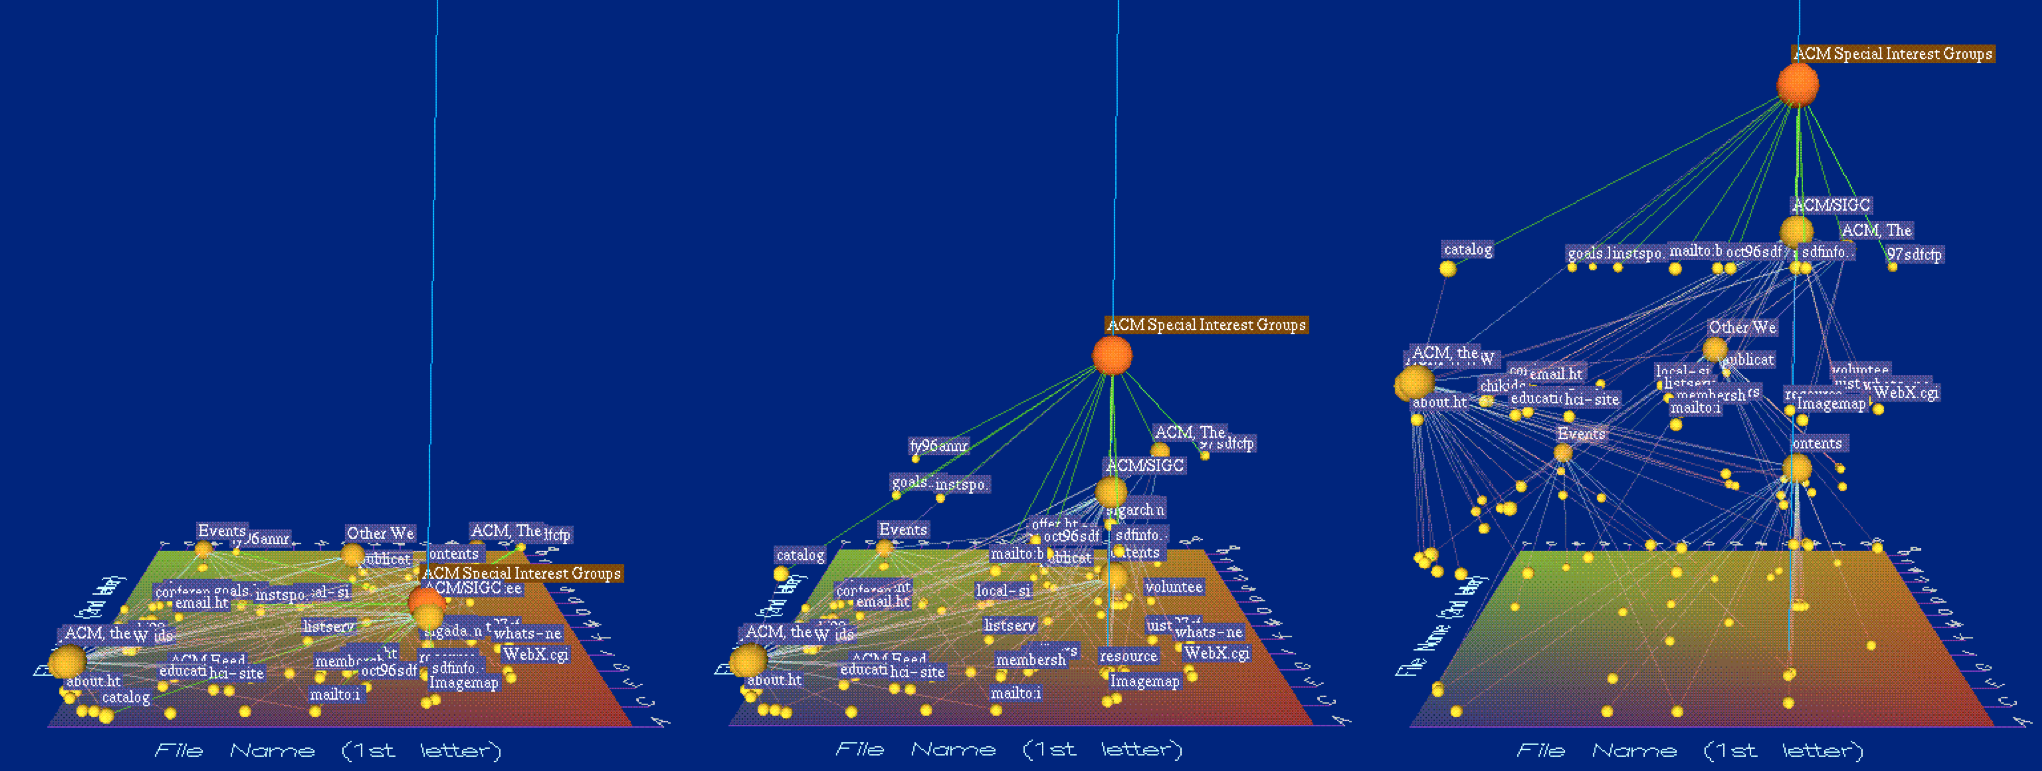
\includegraphics[width=15cm]{natto.eps}
\caption{納豆ビュー}
\label{納豆ビュー}
\end{center}
\end{figure}
UNIXのX-Window System、Mesa、GLUTを用いており、3次元CGグラフ上に展開したノードをリンクに見立て、リンク・被リンクにある関係がエッジで表示される。xy平面には一意的な座標が与えられ、z軸方向にはノードを摘んで持ち上げる、つまりユーザによる操作が可能となっている。これにより、複雑なネットワークをユーザーの意志によってわかりやすく可視化できるようになっている。

\subsection{Flowser}
\begin{figure}[htbp]
\begin{center}
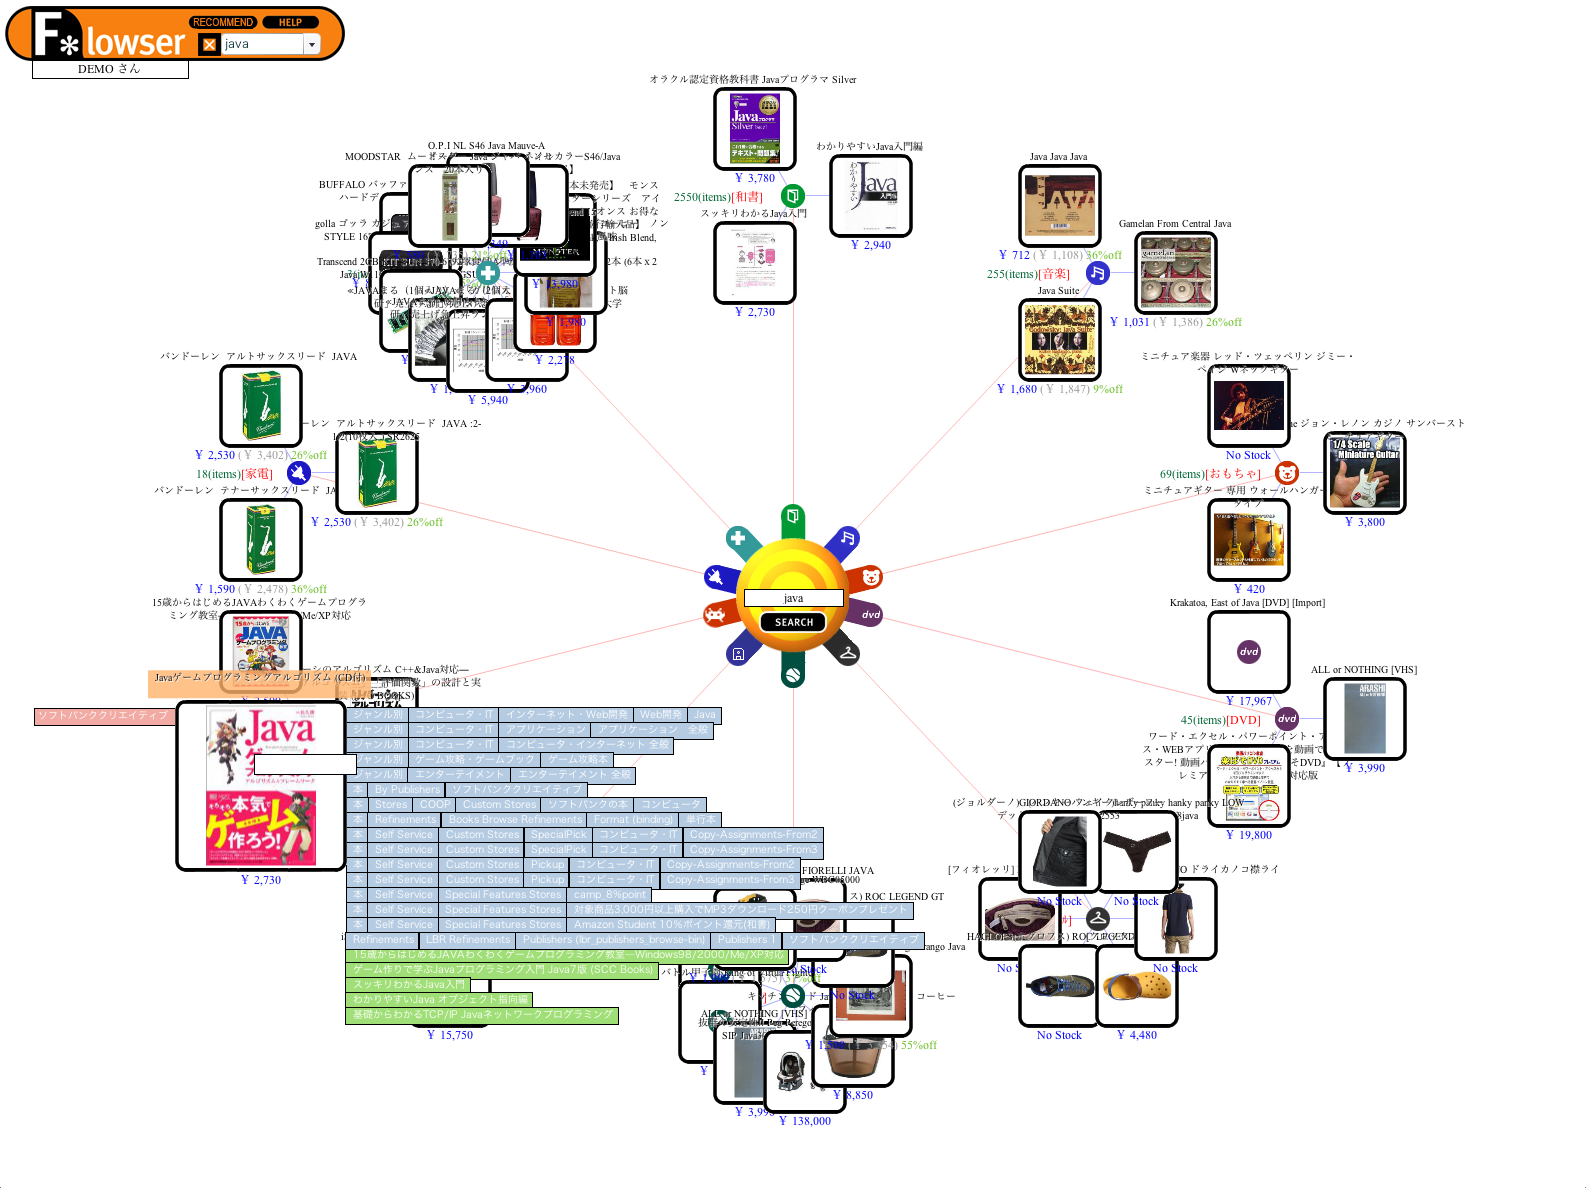
\includegraphics[width=15cm]{flowser.eps}
\caption{Flowser}
\label{flowser}
\end{center}
\end{figure}
Product Advertising APIを用いたWebサービスであり、Mashupの作例でもある。検索ボックスに入力したキーワードからAmazonの複数ジャンルの商品を一気に検索・閲覧することができ、通常のサイトを通じた検索では得られなかった情報を届けることを可能にした。

\section{検索エンジンにおけるWWW視覚化}
以上2つの開発事例を見たところで、改めて、今回の研究で解決したい問題を整理する。
\begin{itemize}
\item タブレットやスマートフォン上から検索結果への直感的な操作
\\
直感的に結果を閲覧するためには、納豆ビューのようにユーザー自身によって結果をわかりやすく可視化できるようにする工夫が必要になる。また、タブレットやスマートフォンでの閲覧を前提とするため、画面サイズやボタンサイズなど、操作性に対する配慮も必要となる。
\\
\item 複数のコンテンツ(検索エンジン)を同時に検索
\\
e-learningコンテンツは、Webページだけでなく、動画、画像、PDFなどの文書ファイルのように、多数の形式に分かれていることが考えられる。であれば、Flowser.comのように、複数結果をそれぞれ分離して見やすく表示する必要がある。
\\
\item e-learningコンテンツへの導線
\\
コンテンツを検索して終了、ではなく、検索したコンテンツへはダイレクトにアクセス可能にする。ページであればブラウザでの表示を行い、動画であればタップと同時に動画サイトやアプリへ遷移し、再生を開始する必要がある。
\end{itemize}

以上の条件から、4つの表示モデルを考えた。

\subsection{Helixモデル}
\begin{figure}[htbp]
\begin{center}
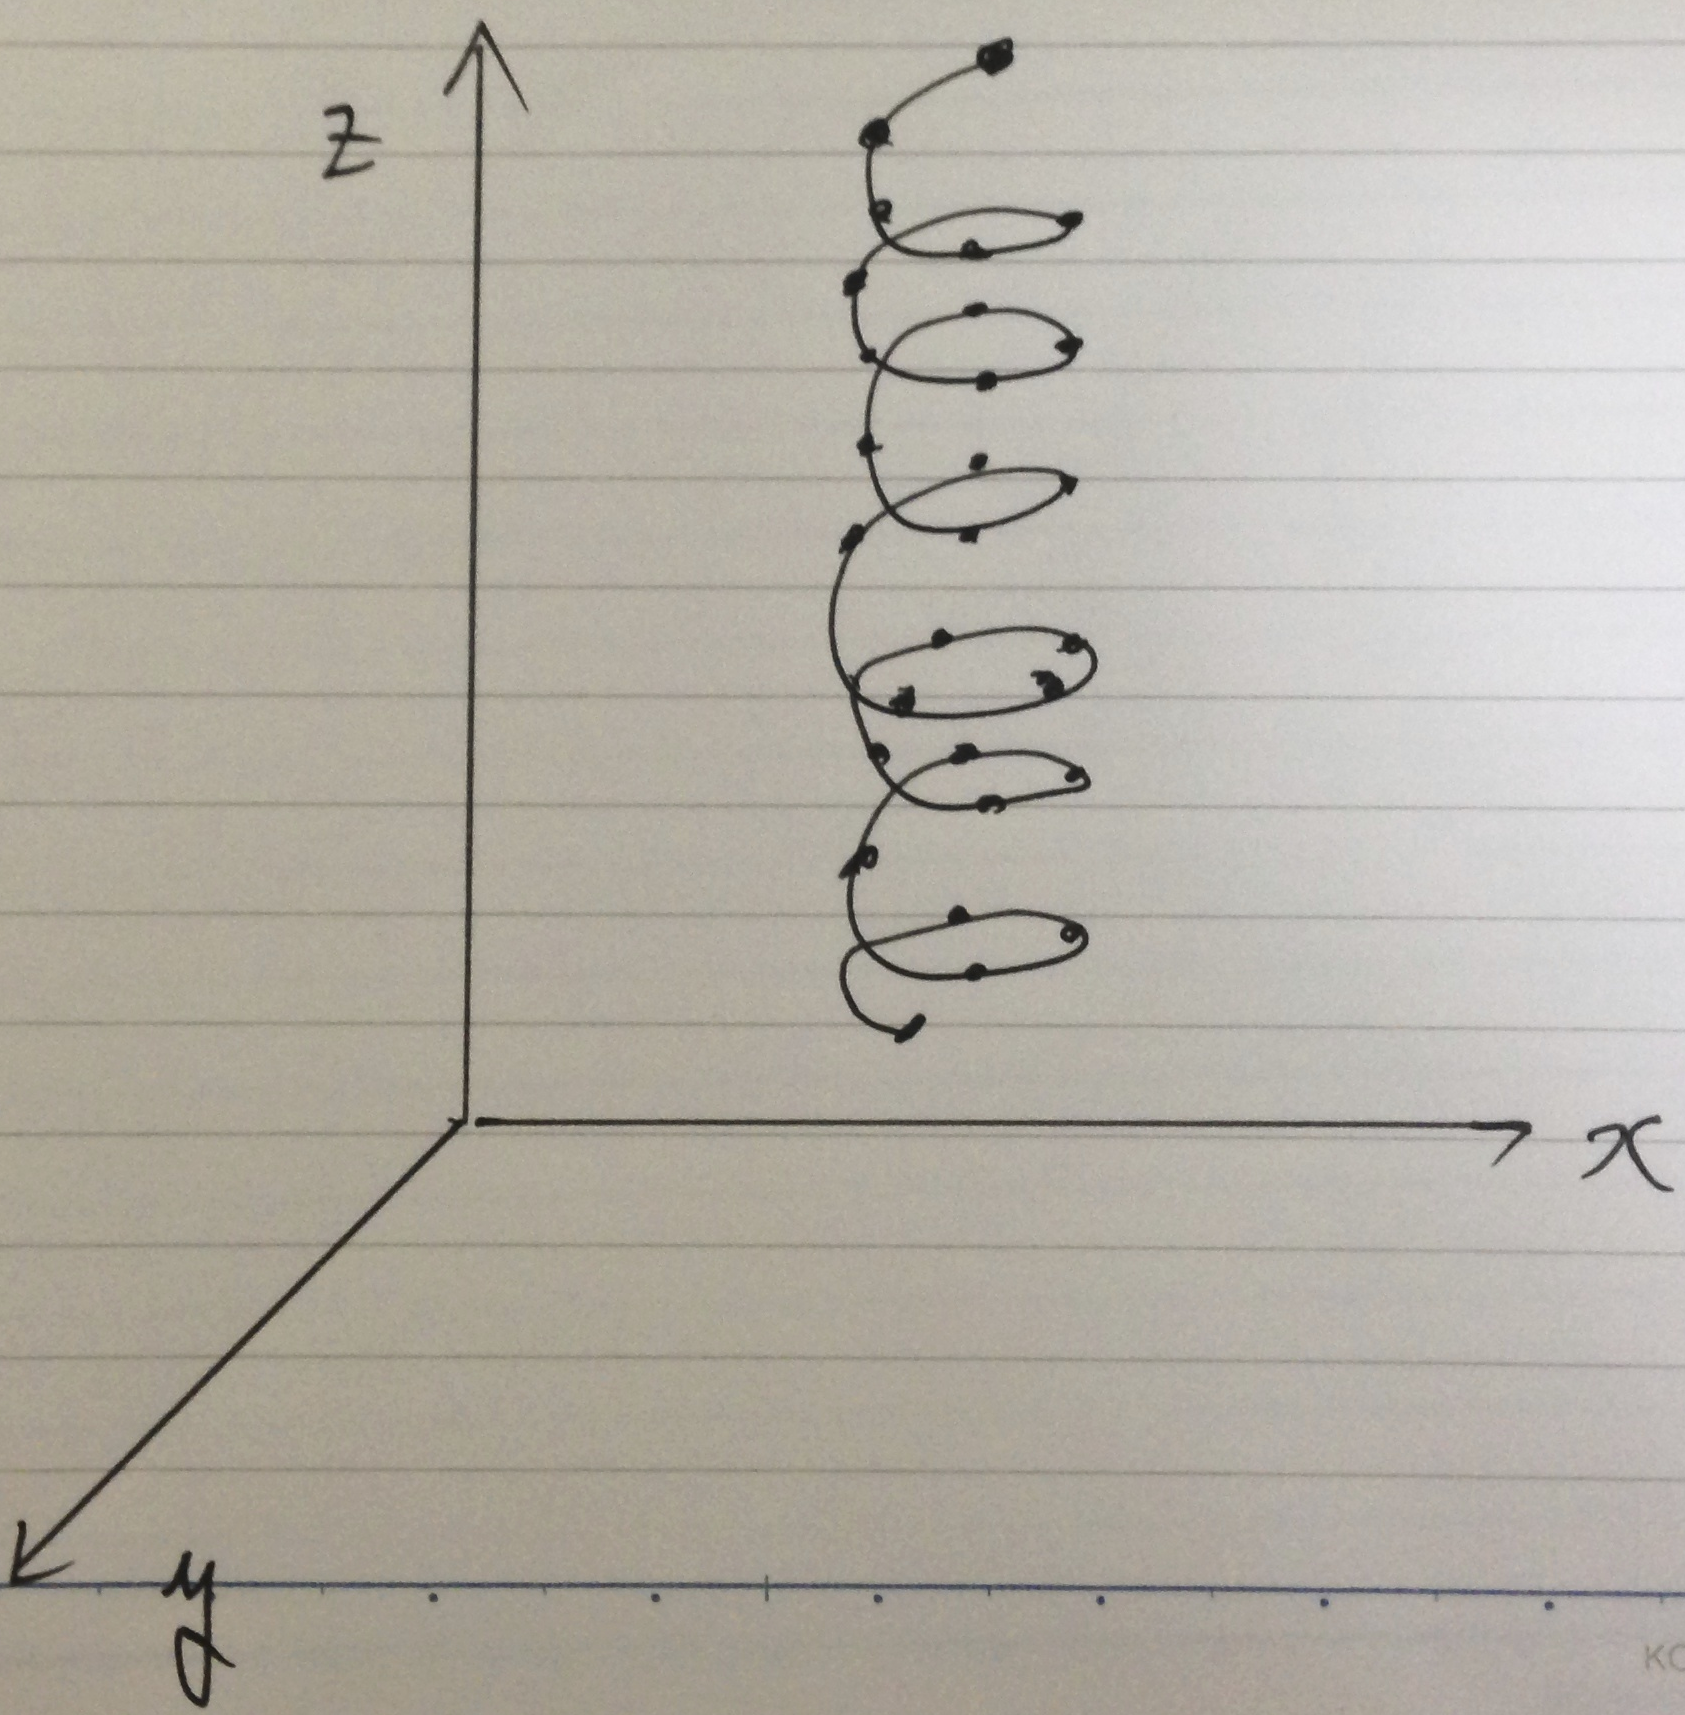
\includegraphics[width=15cm]{helix.eps}
\caption{Helixモデル}
\label{helix}
\end{center}
\end{figure}
3次元螺旋の円周上に検索結果のコンテンツを配置し、螺旋階段を降りるように検索結果の下位コンテンツへと閲覧していくモデルである。この方法の優れた点として、螺旋階段の中心線からコンテンツを見た時、コンテンツ同士の下位と上位が判断しやすく、ユーザがどのような方向にスワイプしても検索結果を辿れる、つまり上下左右方向への持ち替えが容易であるといった利点がある。しかし、複数コンテンツへの対応を考えた際、螺旋一つでは画面上に対しての情報量に無駄が多く、複数コンテンツへ対応しきれない可能性が高いと考えられる。

\subsection{Starモデル}
\begin{figure}[htbp]
\begin{center}
\includegraphics[width=15cm]{star.eps}
\caption{Starモデル}
\label{star}
\end{center}
\end{figure}
複数コンテンツへの配置を最優先に考え、Flowser.comのような円形状のコンテンツ展開を考えたモデルである。コンテンツ毎にそれぞれのノードに分類され、そこから3次元上にランダムにノードが生えており、このノードまでのエッジの長さが検索結果の上位と下位を表している。しかし、3次元上に無作為にノードが存在しているため、コンテンツの一覧性には著しく欠けており、視点を定め辛いことが考えられる。

\subsection{Star-Helixモデル}
\begin{figure}[htbp]
\begin{center}
\includegraphics[width=15cm]{star-helix.eps}
\caption{Star-Helixモデル}
\label{star-helix}
\end{center}
\end{figure}
Helix modelとStar model、両者のメリットをうまく併せて設計したモデルである。螺旋はコンテンツジャンルの数だけ存在し、円形状に展開した始点から同方向に対して一様に伸びている。しかし、複数の螺旋を同時に見れる視点の位置が一意に決まらないため、ユーザーが混乱する可能性が高い。

\subsection{Star-Slideモデル}
\begin{figure}[htbp]
\begin{center}
\includegraphics[width=15cm]{star-line.eps}
\caption{Star-Slideモデル}
\label{star-line}
\end{center}
\end{figure}
Star modelのコンテンツ分離性を活かし、そこから垂直、同方向にコンテンツを配置したモデルである。このモデルを外周から見ると、ちょうど画面上にすべてのコンテンツが入るようになっており、非常に視認性に優れている。加えて、スワイプによって移動する方向も一意であることから、ユーザーが混乱しにくい。また、最前方に配置するコンテンツは丸型ハンガーラックのように回転するようになっており、別のコンテンツをメインに見たい、という時には横方向へのスワイプで自由に切り替えられるようになっている。

\section{採用手法}
以上より、最も多くの問題を改善できた方法として、Star-Slide modelの採用を決定した。	% 本文4
\end{verbatim}
\end{itembox}

目次に続いて、論文のメイン、本文を記述する。アブストラクトと同様で、{\tt main.tex}に直接書くか、\verb|\include| コマンドを利用して別に用意したファイルを{\tt include}する。

本文の書き方は、第\ref{chap:latex}章で詳しく説明する。


\subsection{謝辞の出力}

\begin{itembox}[l]{{\tt main.tex}}
\begin{verbatim}
\begin{acknowledgment}
本研究を卒業論文として完成させることができたのは、担当して頂いた新井康平教授、Herman Tolle博士研究員の熱心なご指導や、第4研究グループの皆様方に協力して頂いたおかげです。皆様へ心より感謝の気持ちと御礼を申し上げたく、謝辞に代えさせていただきます。
\end{acknowledgment}
	% 謝辞。要独自コマンド、include先参照のこと
\end{verbatim}
\end{itembox}

本文のあとには、謝辞を出力する。\verb|begin{acknowledgment}| から \verb|end{acknowledgment}| の間に書いた文章が、謝辞として独立したページに出力される。アブストラクトや本文と同じで、{\tt main.tex}に直接書いてもよいし、\verb|\include| コマンドを利用して{\tt include}してもよい。


\subsection{参考文献の出力}

\begin{itembox}[l]{{\tt main.tex}}
\begin{verbatim}
\begin{bib}[100]


% \bibitem{参照用名称}
%   著者名: 
%   \newblock 文献名,
%   \newblock 書誌情報,出版年.


\bibitem{smartphoneresearch}
\begin{flushleft}
  株式会社シートプランニング:
  \newblock 世界のスマートフォン普及予測
  \newblock {\it http://www.seedplanning.co.jp/press/2012/2012072601.html}, 2012.7.26.
\end{flushleft}

\bibitem{scorm}
\begin{flushleft}
  Advenced Distributed Learning(ADL):
  \newblock SCORM,
  \newblock {\it http://www.adlnet.gov/capabilities/scorm}, 2004.
\end{flushleft}
  
\bibitem{itunesu}
\begin{flushleft}
  Apple,Inc.:
  \newblock iTunes U,
  \newblock {\it http://www.apple.com/jp/education/itunes-u/}, 2004. 
\end{flushleft}

\bibitem{monkasho}
\begin{flushleft}
  文部科学省:
  \newblock 平成十三年文部科学省告示第五十一号(大学設置基準第二十五条第二項の規定に基づく大学が履修させることができる授業等),
  \newblock {\it http://www.mext.go.jp/b\_menu/hakusho/nc/k20010330001/k20010330001.html}, 2001.
\end{flushleft}

\bibitem{docsearch}
\begin{flushleft}
  原真琴:
  \newblock e-learningコンテンツにおけるドキュメントサーチの最適化,
  \newblock 2012.3.
\end{flushleft}

\bibitem{natto}
\begin{flushleft}
  塩澤秀和, 西山晴彦, 松下温:
  \newblock 「納豆ビュー」の対話的 な情報視覚化における位置づけ,
  \newblock 情報処理学会論文誌 Vol.38 No.11, pp.2331-2342, 1997.11.
\end{flushleft}

\bibitem{flowser}
\begin{flushleft}
  有限会社ジャックポット:
  \newblock Flowser,
  \newblock {\it http://flowser.com/}, 2005.4.
\end{flushleft}

\bibitem{away3d}
\begin{flushleft}
  Away3D Team:
  \newblock Away3D,
  \newblock {\it http://away3d.com/}, 2007.
\end{flushleft}

\bibitem{bulkloader}
\begin{flushleft}
  Arthur Debert:
  \newblock Bulk Loader,
  \newblock {\it http://github.com/arthur-debert/BulkLoader}, 2010.
\end{flushleft}

\bibitem{as3crypto}
\begin{flushleft}
  Henri Torgemane:
  \newblock As3 Crypto,
  \newblock {\it http://code.google.com/p/as3crypto/}, 2008.6.
\end{flushleft}

\end{bib}	% 参考文献。要独自コマンド、include先参照のこと
\end{verbatim}
\end{itembox}

謝辞に続いて、参考文献を出力する。

参考文献リストは、\verb|\begin{bib}| から \verb|\end{bib}| の間に、\verb|\bibitem| コマンドを使って書く。文献リストの書き方は、定められたフォーマットがあるわけではなくて、慣例や個々人のこだわりに依るところが多い。ここで示すのは、ぼくが書いた例。

英語の文献の場合、慣例的に書誌名をイタリック体にすることが多いらしい。

\begin{itembox}[l]{{\tt 91\_bibliography.tex}}
\begin{verbatim}
\begin{bib}[100]

% \bibitem{参照用名称}
%   著者名: 
%   \newblock 文献名,
%   \newblock 書誌情報,出版年.

\bibitem{hoge09}
  ほげ山太郎,ほげ山次郎:
  \newblock ほげほげ理論のHCI分野への応用,
  \newblock ほげほげ学会論文誌,Vol.31,No.3,pp.194-201,2009.

\bibitem{hoge08}
  Taro Hogeyama, Jiro Hogeyama:
  \newblock The Theory of Hoge,
  \newblock {\it The Proceedings of The Hoge Society}, 2008.

\end{bib}
\end{verbatim}
\end{itembox}

\verb|\bibitem| コマンド中、参照用名称は、本文から参考文献を参照するときに使うので、忘れずに書いておく。参照文献を本文中に参照するときには、\verb|\cite{参照用名称}| のように書けばよい。例えば、この文の末尾には \verb|\cite{hoge09}| と書いてあるので、自動で対応する番号が振られる\cite{hoge09}。

参考文献リストの番号付けと、本文で参照したときの番号の挿入は、全部が自動で行われる。ただしこれも、第\ref{sec:toc}節で説明した目次の出力と同じで、一時ファイルを生成してからの挿入なので、正しく出力するには最低でも二回のコンパイルが必要。


\subsection{付録の出力}

\begin{itembox}[l]{{\tt main.tex}}
\begin{verbatim}
\appendix
\chapter{プログラム}
実装したActionScriptのソースコード、並びにAndroidアプリを定義するxmlファイルを掲載する。実装はFlashCS6を用いて、Android2.2端末(IS04)での動作を確認している。

\section{main.as(ActionScript)}
\begin{itembox}[l]{{未完成}}
\begin{verbatim}
ギリギリまで粘ったものを添付する予定です……
\end{verbatim}
\end{itembox}

\section{app.xml(XML)}
{\scriptsize
\begin{verbatim}
<?xml version="1.0" encoding="utf-8" standalone="yes"?>
<application xmlns="http://ns.adobe.com/air/application/3.2">
  <id>legdoxea</id>
  <versionNumber>1.0.0</versionNumber>
  <filename>Legdoxea</filename>
  <description>3D view e-learning searcher</description>
  <name>Legdoxea</name>
  <copyright></copyright>
  <initialWindow>
    <content>Legdoxea.swf</content>
    <systemChrome>standard</systemChrome>
    <transparent>false</transparent>
    <visible>true</visible>
    <fullScreen>true</fullScreen>
    <autoOrients>false</autoOrients>
    <aspectRatio>portrait</aspectRatio>
    <renderMode>direct</renderMode>
    <depthAndStencil>true</depthAndStencil>
  </initialWindow>
  <customUpdateUI>false</customUpdateUI>
  <allowBrowserInvocation>false</allowBrowserInvocation>
  <icon></icon>
  <android>
    <manifestAdditions><![CDATA[<manifest>
      <uses-permission android:name="android.permission.INTERNET"/>
    </manifest>]]></manifestAdditions>
  </android>
  <versionLabel></versionLabel>
  <supportedLanguages>en ja</supportedLanguages>
</application>
\end{verbatim}
 }
		% 付録
\end{verbatim}
\end{itembox}

必要であれば、論文の最後には付録を出力する。

\verb|\appendix| コマンド以降に書いたものは、すべて付録として扱われる。付録部分の書き方は通常の本文とまったく同じで、\verb|\appendix| コマンド以降に書くだけで勝手に付録用の体裁で出力される。